\documentclass[a4paper]{jsarticle}
\usepackage[dvipdfmx]{graphicx} % Required for inserting images
\usepackage{amsmath}
\usepackage{amsthm}
\usepackage{amssymb}
\usepackage[margin=20truemm]{geometry}
\usepackage{graphicx}
\usepackage{enumerate}
\usepackage{tikz-cd}
\usepackage{tikz}
\usepackage{mathtools}
\usepackage{trimclip,adjustbox}
\usetikzlibrary{intersections,calc,arrows.meta}

 \theoremstyle{definition}
    \newtheorem{dfn}{定義}[section]
    \newtheorem{prop}[dfn]{命題}
    \newtheorem{lem}[dfn]{補題}
    \newtheorem{thm}[dfn]{定理}
    \newtheorem{cor}[dfn]{系}
    \newtheorem{exam}[dfn]{例}
    \newtheorem{rem}[dfn]{注意}
    \newtheorem{hsk}[dfn]{補足}
    \renewcommand\proofname{\bf 証明}

    \renewcommand{\qedsymbol}{\\Q.E.D}
\newcommand{\SimpComp}{{\mathrm{SimpComp}}}
\newcommand{\Fun}[2]{[#1,~#2]}
\newcommand{\Vect}{{\mathrm{Vect}}}
\newcommand{\SimpCompInc}{{\mathrm{SimpCompInc}}}
\newcommand{\grmodZ}{{\mathrm{grmod \mathbb{Z}_2[x]}}}
\newcommand{\Hom}{{\mathrm{Hom}}}
\newcommand{\ob}{{\mathrm{ob}}}
\newcommand{\Ker}{{\mathrm{Ker}}}
\newcommand{\Image}{{\mathrm{Im}}}

\title{graduate book}
\author{猪原 盛寿}
\date{October 19th 2023}


\begin{document}
\Large
\maketitle
「希望を持ちつつ旅をするのは、そこに行き着くことよりも楽しい」\\
---ロバート・ルイス・ スティーブンソン
\section{導入 Introduction}
本稿はパーシステントホモロジーの代数的解釈について, 暗黙的に用いられている同値関係を圏論によって明示し, より広い応用を支える基礎理論への貢献を試みる. \\

パーシステントホモロジーは位相的データ解析の基本的なツールの一つで, 近年目覚ましい発展を遂げており, その応用範囲はDNAの3次元構造[1]から株式市場[2]に至るまで多岐にわたる. 位相的データ解析では, データ$\Rightarrow$空間$\Rightarrow$代数$\Rightarrow$特徴量という順序で, データから位相・幾何的な構造を抽出した値(特徴量)を算出する[3]. パーシステントホモロジーもこれに習うが, 代数の部分を見る際, 次数付き加群としての解釈とベクトル空間としての解釈の二つが存在する. しばしばこの二つは同値として用いられるが, あくまで暗黙的な了解となっている. そこで次に紹介する圏論を介して明文化することを試みる. \\

直感的なアイデアを他者と共有するには, そのアイデアの形式化を要求される. 概念の形式化とはすなわち数学の仕事であり, 圏論もこれを担う. 数学の中でも特に抽象度の高い圏論では, あらゆる数学的対象を定めた形に書き直すことで, 大域的な関係性を明示する. 例えば, 幾何と代数のような異なる分野の数学的対象の橋渡しも行うことも可能である. \\

本稿の構成は以下の通り. 第2章, パーシステントホモロジーの代数的解釈と圏論の基本的な三つの道具を紹介する. 第3章, パーシステントホモロジーを圏論の観点から記述する. 第4章, 本稿では示しきれなかった課題を記す.
\section{背景 background}
\subsection{パーシステントホモロジー persistent homology}
パーシステントホモロジーに必要な定義を順に記す. 始めは抽象単体複体である. これはデータ$\Rightarrow$空間と変換するためのツールである. 
\begin{dfn}
    抽象単体複体($V,K$)とは, 以下の条件を満たす数学的構造である.\\
    有限集合$V$と$V$の部分集合の有限個の集まり$K$の組($V,K$), から構成され以下の二つの条件を満たす.\\
    \noindent
    (1)$\; \forall v\in V$ならば, $\{v\}\in K$ \\
    (2)$\; \forall a\in K,$かつ $b\subset a$ならば, $b\in K$
\end{dfn}

\begin{exam}
    $V=\{ 1, 2\}, K=\{\{1\}, \{2\}, \{1,2\} \}$とするとき, ($V,K$)は抽象単体複体の定義を満たす. (証明) $V$の部分集合は$\emptyset, \{1\}, \{2\}, \{1,2\}$で$K$は条件を満たす. (1)について, $\{1\}, \{2\}\in K$より満たされる. (2)についても同様. 以上より($V,K$)は抽象単体複体といえる. \\
    また$K'=\{\{1\}, \{1,2\} \}$とするとき, ($V,K'$)は抽象単体複体の定義を満たさない.
\end{exam}
\begin{hsk}
    この定義に従い有限集合であるデータを, 抽象単体複体という構造を持った空間へ変換する. ここで$\sigma=\{v_0,...,v_k\}\in K$を$k$単体と呼び, その次元を$k$で定める. また$K$に含まれる単体の最大次元を, 抽象単体複体($V,K$)の次元と呼び, dim($V,K$)で定める. 上の例では, $\{1\}, \{2\}$を0単体, $\{1,2\}$を1単体と呼び, dim($V,K$)$=1$のようになる.\\
\end{hsk}
抽象単体複体どうしをつなぐ特別な写像の一つに単体写像がある. これは抽象単体複体の構造を保ったまま単体を写す写像である.
\begin{dfn}
    $(V, K), (V', K')$を抽象単体複体とする. 単体写像$f:K\rightarrow K'$とは, $K$の各頂点を$K'$のある頂点に写し以下の条件を満たす写像である.
\begin{equation}
    \forall \{a_0,...,a_q\}\in K\Rightarrow \{f(a_0),...,f(a_q)\}\in K'
\end{equation}
\end{dfn}
\begin{exam}
    $K=\{ \{a\}, \{b\}, \{a,b\}\}, K'=\{ \{x\},\{y\}, \{z\}, \{x,y\}\}$とし, $f:K\rightarrow K'$が$K$の各要素を$f(\{a\})=\{x\}, f(\{b\})=\{y\}$と写すとき, $f$は単体写像の定義を満たす. (証明) $\{f(\{a\}), f(\{b\})\}=\{x,y\}\in K'$より条件を満たすため. \\
    また, $g(\{a\})=\{x\}, g(\{b\})=\{z\}$のとき, $g$は単体写像の定義を満たさない.
\end{exam}
\begin{hsk}
    単体写像は単体を写すのではなく頂点のみを写すことに注意したい. 仮に単体そのものを写す写像を単体写像'とすると, 抽象単体複体の構造を保つことなくその写像は機能を失ってしまう. また, 単体の次元の順序関係を保つ条件として, $\sigma\subseteq\tau \Rightarrow f(\sigma) \subseteq f(\tau)$を加えても次元の順序関係のみが保たれ, 単体としては遥か上の次元へと写すことが可能となってしまう. 結果的に, 抽象単体複体の構造をうまく保つ写像を作ろうとすれば, 上記のように頂点のみを写し条件に単体としての構造が保存されることを加えた定義になるのである. また単体写像はパーシステントホモロジーの代数的解釈に直接関与しないが, 第3章で重要となる定義であるためここで定義した.\\
\end{hsk}

抽象単体複体によってデータ$\Rightarrow$空間と写すことができたが, 次はこの変換によって特徴量が変化しないことを証明する必要がある. その役割を果たすのが脈体定理である.
 
\begin{thm}
    (脈体定理) ([4]定理1.4.1を参照) $X\subset \mathbb{R}^N$が凸閉集合の有限個の集まり$\Phi=\{B_i\subset \mathbb{R}^N| i=1,...,m\}$に被覆されているとする. このとき, 以下の条件を満たす脈体$\mathcal{N}(\Phi)$は, $X$とホモトピー同値となる. 頂点集合を$V=\{1,...,m\}$, 単体の集まり$K$を, 
\begin{equation}
   K = \left\{ \emptyset\neq\sigma\in V \middle| \; \bigcap_{i\in\sigma}^{}B_{i} \neq \emptyset \right\} 
 \notag
 \end{equation}
とすると($\emptyset$ は空集合の意), ($V,K$)は抽象単体複体となる. この抽象単体複体を$\Phi$の脈体と呼び, $\mathcal{N}(\Phi)$で表す.
\end{thm}

\begin{exam}下図は$B_i$を円とするときの脈体の例. 真ん中の穴の情報が保存されていることが分かる.
\end{exam}
\begin{equation}
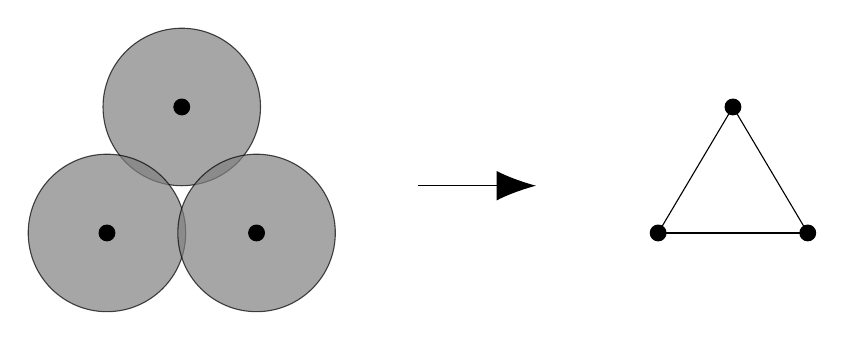
\begin{tikzpicture}
%三つの円%
\filldraw[fill=gray, draw=black, opacity=0.7] (-4,0) circle (1);
\filldraw[fill=gray, draw=black, opacity=0.7] (-4.95,-1.6) circle (1);
\filldraw[fill=gray, draw=black, opacity=0.7] (-3.05,-1.6) circle (1);
%中心点%
\filldraw[fill=black, draw=black] (-4,0) circle (0.1);
\filldraw[fill=black, draw=black] (-4.95,-1.6) circle (0.1);
\filldraw[fill=black, draw=black] (-3.05,-1.6) circle (0.1);
%矢印%
\draw [-{Latex[length=5mm]}]  (-1,-1) -- (0.5,-1);
%三角形%
\filldraw[fill=black, draw=black] (3,0) circle (0.1);
\filldraw[fill=black, draw=black] (3.95,-1.6) circle (0.1);
\filldraw[fill=black, draw=black] (2.05,-1.6) circle (0.1);
\draw (3.95, -1.6) -- (2.05, -1.6);
\draw (3.95, -1.6) -- (3, 0);
\draw (3, 0) -- (2.05, -1.6);
\end{tikzpicture}
\notag    
\end{equation}

\begin{hsk}
$\mathbb{R}^N$は$N$次元ユークリッド空間のこと. 上の図では0単体を頂点, 1単体を頂点を結ぶ線分として表現している. 保存された特徴量は不変量と呼ばれることもある.\\    
\end{hsk}
脈体定理により特徴量を保存したままデータから抽象単体複体へと変換することができた. 次は空間$\Rightarrow$代数へと進むため, 抽象単体複体の代数化に取り組む. \\
\begin{dfn}
($V,K$)を$n$次元抽象単体複体, $m$を$K$内の$k$単体の個数とし, ($V,K$)の$k$単体すべての集まりを$K_k=\{\sigma_1,...,\sigma_m\in K | \; \dim\sigma_i=k \}$とする. このとき$k$鎖群$C_k(K)$は以下で定義する$\mathbb{Z}_2$ベクトル空間である. ($k<0, n<k$のとき, $C_k(K)=0$とする.)
\begin{equation}
   C_k(K)= \mathbb{Z}_2\langle K_k\rangle = \left\{ c=\sum_{i=1}^{m}\alpha_i\sigma_i \middle| \; \alpha_i\in\mathbb{Z}_2 \right\} 
 \notag
\end{equation}
\end{dfn}
\begin{exam}
    $k=2$, $K_2=\{ \{a,b\}, \{b,c\} \}$のとき, $C_2(K)=\{ \{a,b\}, \{b,c\}, \{a,b\}+\{b,c\} \}$となる.
\end{exam}
\begin{hsk}
    $k$鎖群$C_k(K)$は$K_k$から生成される$\mathbb{Z}_2$ベクトル空間と言い換えられる. ここで係数を$\mathbb{Z}_2$に限定した理由は, 同じ単体が現れた際にキャンセルし合うようにするためである($\mathbb{Z}_2$上では1+1=0).\\
\end{hsk}
    $k$鎖群により空間$\Rightarrow$代数へと写すことができた. 次に代数化した$C_k(K)$から特徴量を抽出するため, ここで一つの特別な写像を用意する. これは境界準同型と呼ばれ, 特徴量の定式化に重要な写像である.
\begin{dfn}
  $C_k(K)$の任意の単体を$\sigma=\{v_0,...,v_k\}$とすると, 境界準同型$\partial_k:C_k(K)\rightarrow C_{k-1}(K)$は以下の線形拡張である. 各$0\leq k\leq n$に対して, 
\begin{equation}
    \partial_k(\sigma)=\sum_{j=0}^{k} \{v_0,...,\hat{v_j},...v_k\} \in C_{k-1}(K) \notag
\end{equation}  
(ただし$\{v_0,...,\hat{v_j},...v_k\}$は, $k$単体$\{v_0,...,v_k\}$から$j$番目の$v_j$を除いた$k-1$単体のこと)
\end{dfn}  
\begin{exam}
    $k=1, \sigma=\{v_0,v_1\}$のとき, $\partial_1:C_1(K)\rightarrow C_0(K)$で, $\partial_1(\sigma)=\{v_1\}+\{v_0\}$となり, $k=2, \sigma=\{v_0,v_1,v_2\}$のとき, $\partial_2:C_2(K)\rightarrow C_1(K)$で, $\partial_2(\sigma)=\{v_1,v_2\}+\{v_0,v_2\}+\{v_0,v_1\}$となる. \\
\end{exam}  

  また境界作用素は次の重要な命題を満たす. 
\begin{prop}
    すべての$k\in\mathbb{N}$について$\partial_{k-1}\circ \partial_k=0$が成り立つ. 
\end{prop}
\begin{proof}
    $\sigma_i=\{v_0,...,v_k\}$とすると, 
\begin{equation}
    \begin{array}{lll}
       \partial_{k-1}\circ \partial_k(\sigma_i)  & = & \partial_{k-1}(\sum\limits_{j=0}^{k} \{v_0,...,\hat{v_j},...v_k\})\\
         & = & \sum\limits_{j=0}^{k}  \partial_{k-1}(\{v_0,...,\hat{v_j},...v_k\})\\
         & = & \sum\limits_{j=0}^{k}  (\sum\limits_{l<j}^{} \{v_0,...,\hat{v_l},...,\hat{v_j},...v_k\}\\
         & & +\sum\limits_{l>j}^{} \{v_0,...,\hat{v_j},...,\hat{v_l},...v_k\})\\
         & = & \sum\limits_{l<j}^{} \{v_0,...,\hat{v_l},...,\hat{v_j},...v_k\}\\
         & & +\sum\limits_{l>j}^{} \{v_0,...,\hat{v_j},...,\hat{v_l},...v_k\}\\
         & = & 0 \notag
    \end{array}
\end{equation} \\
\end{proof}
\begin{hsk}
    $\mathbb{Z}_2$ベクトル空間での計算であるため, 同じ元どうしの和は互いにキャンセルされ0になる. また, 上の命題は$\partial_k$ の核と$\partial_{k+1}$の像の包含関係を意味する:
\begin{equation}
    \begin{array}{lll}
        &  & \Ker \partial_k =\{c \in C_k(K)| \partial_k(c)=0\}\\
         & \supset & \Image \partial_{k+1} = \{c \in C_k(K)| c= \partial_{k+1}(c'), c'\in C_{k+1}(K)\}\notag
    \end{array}
\end{equation}\\
\end{hsk}
境界準同型によって$k$鎖群の各次元は繋がれ下図の系列が表れる. 
\begin{equation}
    0\rightarrow C_n(K)\xrightarrow[]{\partial_n} C_{n-1}(K)\xrightarrow[]{\partial_{n-1}}\cdot\cdot\cdot\xrightarrow[]{\partial_2} C_1(K)\xrightarrow[]{\partial_1} C_0(K)\rightarrow 0\notag
\end{equation}


\begin{dfn}
    $K$を抽象単体複体とし, $Z_k(K)=\Ker \partial_k, B_k(K)=\Image \partial_{k+1}$とすると, ホモロジー群$H_k(K)$は以下の式で表される.
    \begin{equation}
        H_k(K)=Z_k(K)/B_k(K)\notag
    \end{equation}
\end{dfn}
このホモロジー群と次に紹介するフィルトレーションにより, 特徴量の定式化であるパーシステントホモロジーが定義できる.  
\begin{dfn}
    $K$を抽象単体複体とする. $K$のフィルトレーションとは, 
    \begin{equation}
        \mathbb{K}: K^0\subset K^1\subset \cdot\cdot\cdot\subset K^t\subset \cdot\cdot\cdot \notag
    \end{equation}
    のことである. ここで$t$は時刻と呼ぶことにする.
\end{dfn}
また, 各時刻のホモロジー群をつなぐ線形写像を次のように定義する.
\begin{dfn}
    $H_k(K^t)$の任意の単体を$z$を用いて, $\varphi_k:H_k(K^t)\rightarrow H_k(K^{t+1})$は以下のように定義する写像である.
    \begin{equation}
    \begin{array}{cccc}
         \varphi_k:& H_k(K^t) & \longrightarrow & H_k(K^{t+1}) \\
        & \rotatebox{90}{$\in$} & & \rotatebox{90}{$\in$} \\
        & [z] & \longmapsto & [f_k(z)]\notag
    \end{array}
\end{equation}
     $f_k$は単体写像$f:K^t\rightarrow K^{t+1}$が誘導する鎖群の線形写像$f_k:C_k(K^t)  \rightarrow C_k(K^{t+1})$であり, 次のように定める.
\begin{equation}
    f_k(\{ a_0,...,a_k\})=\left\{
    \begin{array}{c l}	
    \{ f(a_0),...,f(a_k)\} & (f(a_0),...,f(a_k)が相異なるとき)\\
    0 & (そうでないとき)\notag
\end{array}\right.
\end{equation}\\
\end{dfn}
これにより, 次のホモロジー群と線形写像の列が生成され, これをパーシステントホモロジーと呼ぶ.
\begin{dfn}
    フィルトレーション$K$の$k$次パーシステントホモロジーとはホモロジー群と線形写像の族の組
    \begin{equation}
     H_k(K^0)\rightarrow H_k(K^1)\rightarrow \cdot\cdot\cdot\rightarrow H_k(K^t)\rightarrow \cdot\cdot\cdot\notag
\end{equation}
のことである.\\
\end{dfn}

以上がベクトル空間でのパーシステントホモロジーである. 一方で, もう一通りのパーシステントホモロジーの定義が存在する. 上では$C_k(K)$をベクトル空間として定義したが, 次は$C_k(\mathbb{K})$を次数付き$\mathbb{Z}_2[x]$加群として定義する. \\
ではまず, 次数付き$\mathbb{Z}_2[x]$加群とそれらをつなぐ写像について記す.

\begin{dfn}
    次数付き$\mathbb{Z}_2[x]$加群$M$とは, $\mathbb{Z}_2[x]$加群である$M$にアーベル群としての直和分解を与え, $x^jM_i\subset M_{i+j}$を満たすものである($i,j\in\mathbb{N}_0$).
    \begin{equation}
        M=\bigoplus_{i=0}^{\infty} M_i\notag
    \end{equation}\\
\end{dfn}
\begin{dfn}
    $\mathbb{Z}_2[x]$準同型写像とは, $M, N$を$\mathbb{Z}_2[x]$加群とすると, $f:M\rightarrow N$が次の条件を満たすものである. $(a, b\in M)$
        \begin{flalign}
             &(1) f(a+b) = f(a)+f(b)& \notag \\
             &(2) f(xa)= xf(a)& \notag
        \end{flalign}
\end{dfn}

\begin{dfn}
    次数付き$\mathbb{Z}_2[x]$準同型写像とは, $M, N$を次数付き$\mathbb{Z}_2[x]$加群とすると, $f:M\rightarrow N$が$\mathbb{Z}_2[x]$準同型写像であって, $f(M_i)\subset N_i$を満たすものである.\\
\end{dfn}
ここで$C_k(\mathbb{K})$を次数付き$\mathbb{Z}_2[x]$加群として定義する.
\begin{dfn}
    ($V,K$)を$n$次元抽象単体複体, $K^t$の任意の単体を$\sigma$とし, $C_k(K^t)$を
    \begin{equation}
        C_k(K^t)=\sum_{\sigma\in K_k^t}^{} \mathbb{Z}_2 \sigma \notag
    \end{equation}
    とすると, これらの直和$C_k(\mathbb{K})$は以下で定義する次数付き$\mathbb{Z}_2[x]$加群である.
    \begin{equation}
        C_k(\mathbb{K})=\bigoplus_{t\geq 0}^{}C_k(K^t)=\{(c_0, c_1, \cdot\cdot\cdot,c_t, \cdot\cdot\cdot)\;|\;c_t\in C_k(K^t) \} \notag
    \end{equation}
    $x$の作用は以下に定める.
    \begin{equation}
        x \cdot (c_0, c_1, \cdot\cdot\cdot)= (0, c_0, c_1, \cdot\cdot\cdot) \notag
    \end{equation}\\
\end{dfn}
そして次数付き$\mathbb{Z}_2[x]$準同型写像である境界準同型により, 前回同様$C_k(\mathbb{K})$の各次元をつないだ下図の系列が表れる.
\begin{equation}
    0\rightarrow C_n(\mathbb{K})\xrightarrow[]{\partial_n} C_{n-1}(\mathbb{K})\xrightarrow[]{\partial_{n-1}}\cdot\cdot\cdot\xrightarrow[]{\partial_2} C_1(\mathbb{K})\xrightarrow[]{\partial_1} C_0(\mathbb{K})\rightarrow 0\notag
\end{equation}
$Z_k(\mathbb{K})=\Ker \partial_k, B_k(\mathbb{K})=\Image \partial_{k+1}$とすると, どちらも次数付き$\mathbb{Z}_2[x]$加群であるから$Z_k(\mathbb{K})=\bigoplus_{t\geq 0}^{}Z_k(K^t), B_k(\mathbb{K})=\bigoplus_{t\geq 0}^{}B_k(K^t)$と表すことができる.\\
これらを用いて, パーシステントホモロジーは定義される.
\begin{dfn}
    $K$のフィルトレーション$\mathbb{K}$に対して, $k$次パーシステントホモロジー$PH_k(\mathbb{K})$は以下の次数付き$\mathbb{Z}_2[x]$加群である.
    \begin{equation}
        PH_k(\mathbb{K})=Z_k(\mathbb{K})/B_k(\mathbb{K})\notag
    \end{equation}
\end{dfn}
これは別の表現で,
\begin{equation}
        PH_k(\mathbb{K})=\bigoplus_{t\geq 0}^{}Z_k(K^t)/B_k(K^t)=\bigoplus_{t\geq 0}^{}H_k(K^t)
        \notag
\end{equation}
となり, 直和された各時刻のホモロジー群は準同型写像$\varphi_t^{t+1}:H_k(K^t)\rightarrow H_k(K^{t+1})$によりつながれる. ($\varphi_t^{t+1}([z])=x\cdot [z]$)\\
ここまで二通りのパーシステントホモロジーを定義した. これを次に紹介する圏論を用いてその関係性を第3章で明らかにする.

\subsection{圏論 category theory}
数学には, 「関係性」に着目した極めて抽象的な分野が存在する. それは圏論である. ここからは圏論の基本的な三つの道具(圏, 関手, 自然変換)を定義し, 第3章へとつなげたい. 手始めに, 圏(category)の定義を確認する.
\begin{dfn}
圏$X$とは以下の条件を満たす数学的構造である. 
\begin{itemize}
    \item 対象(object)の集まり ob($X$)
    \item 各対象$A, B$に対して$A$から$B$への射の集まり Hom($A, B$)
    \item 射の合成と呼ばれる関数$(\circ)$
\end{itemize}
\begin{equation}
    \begin{array}{lllll}
     \circ &: \Hom (B, C) &\times \Hom (A, B) &\rightarrow &\Hom (A, C)  \\
         &    & (g,f) & \mapsto&  g\circ f
\end{array}
\end{equation}
から構成され, 射は次の二つの法則を満たす.
\begin{enumerate}[(1)]
    \item 結合法則. 任意の射$f\in \Hom(A,B), g\in \Hom(B,C), h\in \Hom(C,D),$は次の等式を満たす. $(h \circ g) \circ f = h \circ (g \circ f)$  
    \item 単位法則. 任意の対象$A$に対し, 恒等射と呼ばれる射$1_A:A\rightarrow A$が存在し, 次の等式を満たす.  $f\circ 1_A = 1_B\circ f = f$  
\end{enumerate}
\begin{equation}
    \begin{tikzcd}
    A\ar{r}{f} \ar[loop left,"1_A"] \ar[bend right=30,swap]{rr}{g\circ f}& B\ar{r}{g} \ar[bend left=30]{rr}{h\circ g}& C\ar{r}{h} & D
\end{tikzcd}
\end{equation}
\end{dfn}

\begin{hsk}
まとめると圏とは, 対象, 射, 射の合成からなり, 射が二つの法則を満たすものである.
対象とは, 集合でいうところの要素のこと. A, ☆, 1, 〇, ...など集合や数字に限らない.
射とは, 対象間に走る矢印のこと.対象同士を結ぶこと, 向きが存在すること, が条件となる. $A \rightarrow B$, 〇$\rightarrow$☆, などで$A$と$B$の間の射は一本とは限らない. このときのA, 〇を始域といい, 反対にB, ☆は終域という. 圏論が「関係性」の数学と呼ばれるように, 圏では射が主役となる. 構成要素の一つに射の合成が入っている. 片方の終域ともう片方の始域が一致するとき, 二つを合成した射が一つ存在する. 結合法則や単位法則は, 写像のそれと同様である. 
\\
\end{hsk}

\begin{exam}
対象を1,2,...の自然数全体, 射を$m\leqq n$ならば$m \rightarrow n$ ($m, n \in \mathbb{N}$)とする集まり$C$を考える.\\ ob($C$)$= \mathbb{N}$. $m\leqq n$のとき$\Hom (m, n)=\{m\rightarrow n\}$. $m>n$のとき$\Hom (m, n)=\{\}$. $l, m, n\in$ ob$(X)$, $l \rightarrow m \rightarrow n$ならば, $l\leqq m\leqq n$から$l\leqq n$より$l \rightarrow n$. よって射の合成は含まれている. 次に射が二つの法則を満たすか確認する. 
 \begin{enumerate}[(1)]
        \item $k\rightarrow l\rightarrow m\rightarrow n$ならば, 合成により$k\rightarrow m$, $l \rightarrow n$が存在し, さらに二つの射を利用し同じ射$k\rightarrow n$が合成できる. よって射は結合法則を満たす.
        \item $m\rightarrow n$ならば, $m\leqq m$より$m\rightarrow m$が存在し, $m\rightarrow m\rightarrow n$と$m\rightarrow n\rightarrow n$から同じ射$m\rightarrow n$が合成できる. よって, 射は単位法則を満たす.
\end{enumerate}
以上より, $C$は圏と定義できる.\\
\end{exam}
圏を定義出来たおかげで,対象と対象の関係性が射によって表せられるようになった. では圏と圏の関係性を表すときはどうすればよいだろうか?答えはシンプルで, もう一度射を伸ばせばよい. 圏論ではその射を, 「関手(functor)」と呼ぶ.
\begin{dfn}
    $X, Y$を圏とする. 関手$F:X\rightarrow Y$は, 
    \begin{itemize}
        \item 対象についての関数:ob$(X)\rightarrow$ ob$(Y)$  $\; [A\mapsto F(A)]\;(\forall A\in\ob(X))$ 
        \item 射についての関数:$\Hom (A, B)\rightarrow \Hom (F(A), F(B))$  $\; [f\mapsto F(f)]\; \;(\forall A, B\in\ob(X))$
    \end{itemize}
からなり, 射についての関数が次の二つの公理を満たす.
    \begin{itemize}
        \item[(1)] 圏$X$で, $A\xrightarrow[]{f} B\xrightarrow[]{g} C$のとき, $F(g\circ f) = F(g)\circ F(f)$
        \item[(2)] $A\in$ob$(X)$のとき, $F(1_A) = 1_F(A)$
    \end{itemize}
\begin{equation}
    \begin{array}{llll}
         F:& X & \longrightarrow & Y \\
        & \rotatebox{90}{$\in$} & & \rotatebox{90}{$\in$} \\
        \mbox{対象}:& A & \longmapsto & F(A)\\
         \mbox{ 射}:& f & \longmapsto & F(f)\\
    \end{array}
\end{equation}
\end{dfn}

\begin{hsk}
    関手とは, 圏と圏の間の射である. 対象と射についての関数(射)で構成し, (1)で合成を(2)で単位法則を保存する. 準同型写像がその構造を保つように, 関手は圏としての構造を保つ射である. 以降は, 記号や矢印が増えるためメモ等で図を書くことをお願いしたい.\\
\end{hsk}

ここで, 第3章で重要となる特殊な関手について定義しておく.
\begin{dfn}
    関手$F:X\rightarrow Y$は, 任意の対象$A, A'\in \ob(X)$について
\begin{equation}
    \begin{array}{cccc}
         F:& \Hom(A, A') & \longrightarrow & \Hom(F(A), F(A')) \\
        & \rotatebox{90}{$\in$} & & \rotatebox{90}{$\in$} \\
        & f & \longmapsto & F(f)\notag
    \end{array}
\end{equation}
が単射であるとき忠実であり, 全射であるとき充満と呼ぶ. 忠実かつ充満である関手を忠実充満関手という.\\
\end{dfn}


関手のおかげで圏と圏の関係性を表せられるようになった. では関手と関手の関係性を表すときはどうすればよいだろうか?察しの良い読者はもうお気づきだろうが答えはやはりシンプルである. もう一度だけ射を伸ばそう, 圏論ではその射を「自然変換(natural transformation)」と呼ぶ.
\begin{dfn}
    $X, Y$を圏, $F, G$を$X$から$Y$への関手, とする.\\
    $F$から$G$への自然変換$\alpha$とは,
    \begin{itemize}
        \item $Y$の射の族 ($F(A)\xrightarrow[]{\alpha_A} G(A)$, $A\in\ob(X)$)
    \end{itemize}
    からなり, この射の族が次の等式を満たす.
    \begin{itemize}
        \item $A, B\in\ob(X), A\xrightarrow[]{f}B$ならば, $\; G(f)\circ \alpha_A = \alpha_B\circ F(f)$
    \end{itemize}
\end{dfn}
\begin{equation}
\begin{tikzcd}
X
\arrow[r, bend left, "F"]
\arrow[r, bend right, swap, "G"]
\arrow[r, phantom, bend left, shift right=0.2ex, ""{name=U}]
\arrow[r, phantom, bend right, shift left=0.2ex, swap, ""{name=D}]
&Y
\arrow[Rightarrow, from=U, to=D, "\alpha"]
\end{tikzcd}
     \begin{tikzcd}
        F(A)\arrow{r}{F(f)} \arrow{d}{\alpha_A} & F(B)\arrow{d}{\alpha_B}\\
        G(A)\arrow{r}{G(f)} & G(B)
    \end{tikzcd}
\end{equation}
\begin{hsk}
    自然変換とは関手と関手の間の射である. 対象についての関数で写された対象同士を結ぶ射で構成する. よってその射の全ては, 関手の終域の圏に帰属する. 満たされるべき等式は, 射についての関数で写された射と自然変換の射について条件を課すものである. 上記右側の図において, $F(A)\rightarrow G(B)$について二通りの合成が可能となる. その二つの合成射が一致する必要が自然変換にはある.\\
\end{hsk}



\section{結果 Result}
パーシステントホモロジーの圏論的解釈を下図に表す. 
\begin{equation}
    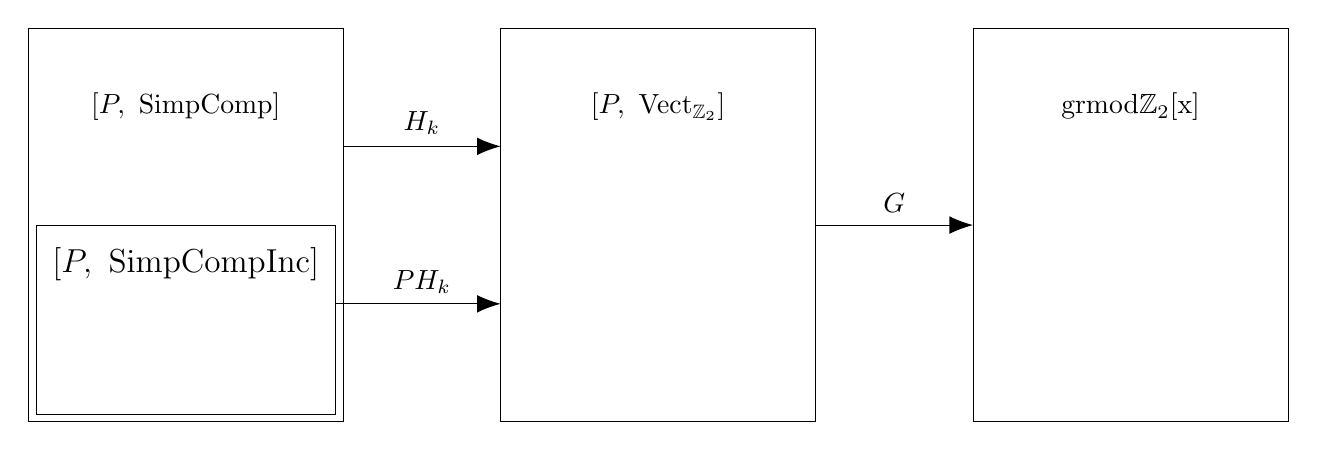
\begin{tikzpicture}
    \node at (-6, 1) {$\Fun{P}{\SimpComp}$};
    \node at (-6, -1) {{\large$\Fun{P}{\SimpCompInc}$}};
    \node at (0, 1) {$\Fun{P}{\Vect_{\mathbb{Z}_2}}$};
    \node at (6, 1) {$\grmodZ$};
    \node at (-3, 0.8) {$H_k$};
    \node at (3, -0.22) {$G$};
    \node at (-3, -1.22) {$PH_k$};
    \draw (-2,-3) rectangle (2,2);
    \draw (4,-3) rectangle (8,2);
    \draw (-8,-3) rectangle (-4,2);
    \draw (-7.9,-2.9) rectangle (-4.1,-0.5);
    \draw [-{Latex[length=3mm]}]  (-4,0.5) -- (-2, 0.5);
    \draw [-{Latex[length=3mm]}]  (-4.1,-1.5) -- (-2, -1.5);
    \draw [-{Latex[length=3mm]}]  (2,-0.5) -- (4, -0.5);
\end{tikzpicture}\notag
\end{equation}

次に詳細な圏や関手の定義を記す.
\begin{prop}
    対象を抽象単体複体, 射を単体写像とする圏, $\SimpComp$が存在する
\end{prop}
\begin{proof}
    単体写像どうしの合成が, 再び単体写像になるか確認する. $f:K\rightarrow K'$, $f':K'\rightarrow K''$を単体写像とすると
{\large
\begin{equation}
    \begin{array}{ll}
        \forall\sigma =\{a_0,...,a_q\}\in K & \Rightarrow \{f(a_0),...,f(a_q)\}\in K'\Rightarrow\{f'(f(a_0)),...,f'(f(a_q))\}\in K'' \\
         &  \Rightarrow\{f'\circ f(a_0),...,f'\circ f(a_q)\}\in K''\notag
    \end{array}
\end{equation}
}
となるため, これは定義を満たし, $f'\circ f:K\rightarrow K''$は単体写像となる. 次に$K\xrightarrow[]{f} K'\xrightarrow[]{g} K''\xrightarrow[]{h}K'''$のとき, $K$の任意の頂点$a_i$について
\begin{equation}
    \begin{array}{ll}
        (h\circ g)\circ f(a_i) & =(h\circ g)(f(a_i))=h\circ g\circ f(a_i) \\
        h\circ (g\circ f)(a_i) & =h(g\circ f(a_i))=h\circ g\circ f(a_i)\notag
    \end{array}
\end{equation}
より, $(h\circ g)\circ f=h\circ (g\circ f)$となって結合法則が満たされる. また$1_K:K\rightarrow K, 1_{K'}:K'\rightarrow K'$のとき, $f\circ 1_K(a_i)=f(a_i)$かつ$1_{K'}\circ f(a_i)=1_{K'}(f(a_i))=f(a_i)$より, $f\circ 1_K=1_{K'}\circ f=f$となって単位法則も満たされた. 以上より, SimpCompは圏である.\\
\end{proof}


\begin{lem}
    対象を$\mathbb{Z}_2$ベクトル空間, 射を線形写像とする圏, $\Vect_{\mathbb{Z}_2}$が存在する
\end{lem}
\begin{proof}
    線形写像の合成が線形写像になるか確認する. $f:V\rightarrow V'$, $f':V'\rightarrow V''$を線形写像とし, $a, b$をスカラー, $x, y\in V$とすると, 
\begin{equation}
    \begin{array}{ll}
        f'\circ f(ax+by) & =f'(af(x)+bf(y))=af'(f(x))+bf'(f(y)) \\
         & =a(f'\circ f)(x)+b(f'\circ f)(y)\notag
    \end{array}
\end{equation}
となるため, これは定義を満たし$f'\circ f:V\rightarrow V''$も線形写像となる. 結合法則, 単位法則については上と同様. 以上より$\Vect_{\mathbb{Z}_2}$は圏である.\\
\end{proof}



\begin{prop}
    $H_k:\SimpComp \rightarrow \Vect_{\mathbb{Z}_2}$を次のように定義するとき, これは関手となる. $K, K'$を抽象単体複体として, 二つの関数ob$(\SimpComp)\rightarrow$ ob$(\Vect)$, $\Hom (K, K')\rightarrow \Hom (H_k(K), H_k(K'))$からなり, $f\in \Hom(K, K')$のとき$H_k(f)$は定義2.19と同様に定める.
\end{prop}
\begin{proof}
    $H_k$が関手となるため満たすべき条件は二つ. (1)$K\xrightarrow[]{f}K'\xrightarrow[]{f'}K''$ならば, $H_k(f'\circ f) = H_k(f')\circ H_k(f)$. (2) $1_K:K\rightarrow K$ならば, $H_k(1_K)=1_{H_k(K)}$. $K\xrightarrow[]{f}K'\xrightarrow[]{f'}K''$のとき, $H_k(f')\circ H_k(f)([z]) = H_k(f')([f_k(z)]) = [f'_k\circ f_k(z)]$となり, 他方$H_k(f'\circ f) ([z])  = [ (f'\circ f)_k(z)]$となるため, (1)を示すためには$f'_k\circ f_k=(f'\circ f)_k$の確認が急務となる.
\begin{equation}
    f'_k\circ f_k(\{ a_0,...,a_k\})=\left\{
    \begin{array}{c l}	
    f'_k(\{ f(a_0),...,f(a_k)\}) & (f(a_0),...,f(a_k)が相異なるとき)\\
    f'_k(0) & (そうでないとき)\notag
\end{array}\right.
\end{equation}
であり, さらに{\large
\begin{equation}
    f'_k(\{ f(a_0),...,f(a_k)\})=\left\{
    \begin{array}{c l}	
    \{ f'\circ f(a_0),...,f'\circ f(a_k)\} & (f'\circ f(a_0),...,f'\circ f(a_k)が相異なるとき)\\
    0 & (そうでないとき)\notag
\end{array}\right.
\end{equation}}
    $f$は単体写像であるため$f'_k(0)=f(0)=0$となる. よって, {\large
\begin{equation}
    f'_k\circ f_k(\{ a_0,...,a_k\})=\left\{
    \begin{array}{c l}	
    \{ f'\circ f(a_0),...,f'\circ f(a_k)\} & (f'\circ f(a_0),...,f'\circ f(a_k)が相異なるとき)\\
    0 & (そうでないとき)\notag
\end{array}\right.
\end{equation}}

と書くことができる. そしてこれは定義から$(f'\circ f)_k(\{ a_0,...,a_k\})$と等しいため, $f'_k\circ f_k=(f'\circ f)_k$がいえる. よって(1)の$K\xrightarrow[]{f}K'\xrightarrow[]{f'}K''$ならば, $H_k(f'\circ f) = H_k(f')\circ H_k(f)$は満たされた.\\
    次に$1_K:K\rightarrow K$のとき, $H_k(1_K):H_k(K)\rightarrow H_k(K)$で$H_k(1_K)([z])=[1_K(z)]=[z]$となる. これは恒等写像の性質を満たすため, $H_k(1_K)=1_{H_k(K)}$がいえる. よって(2)も満たすことができたので, $H_k:\SimpComp\rightarrow \Vect_{\mathbb{Z}_2}$は関手である. \\
\end{proof}


これをホモロジー関手と呼ぶ. では次に数字を割りあてた単体複体からのホモロジー関手を考える.
\begin{cor}
    対象を1,2,...,nの自然数, 射を$i \leq j$ ならば,  $i\rightarrow j(i, j \in \mathbb{N})$とする圏, $P$が存在する
\end{cor} 
\begin{lem}
    対象を$P$から$\SimpComp$への関手, 射を自然変換とする圏, $\Fun{P}{\SimpComp}$が存在する.
\end{lem}
\begin{proof}
    いくつかの条件を満たし$P$から$\SimpComp$への関手は定義できる. 自然変換は, 圏$\SimpComp$の射で構成されるため, 射の合成の存在と射が満たすべき二つの法則は満たされる. 以上から$\Fun{P}{\SimpComp}$を圏として定義することができる.\\
\end{proof}
同様に$\Fun{P}{\Vect_{\mathbb{Z}_2}}$も圏である. これを$P$との関手圏と呼ぶことにする. この二つの圏の間の関手$H_q:\Fun{P}{\SimpComp}\rightarrow \Fun{P}{\Vect_{\mathbb{Z}_2}}$は,
\begin{equation}
    \begin{array}{cccc}
         H_q:& \Fun{P}{\SimpComp} & \longrightarrow & \Fun{P}{\Vect_{\mathbb{Z}_2}} \\
        & \rotatebox{90}{$\in$} & & \rotatebox{90}{$\in$} \\
        & \mathbb{K}& \longmapsto & H_q(\mathbb{K})\\
         & =\{K_0\rightarrow ...\rightarrow K_n\} &  & =\{Hq(K_0)\rightarrow ...\rightarrow H_q(K_n)\}\\
    \end{array}
\end{equation}
のようになり, 前項で定義したようにこの関手は単体複体からホモロジーを計算することを表している. $P$との関手圏にすることで, 列ごとの計算に拡張できた. しかし, SimpCompの射は単体写像であるためこのままでは単なる列である. 
そこでさらに, $\SimpComp$からフィルトレーションのみを抽出するため, 射を包含写像に限定した$\SimpCompInc$を定義する. 
\begin{cor}
    対象を単体複体, 射を包含写像とする圏, $\SimpCompInc$は$\SimpComp$の部分圏であり, $\Fun{P}{\SimpCompInc}\subset \Fun{P}{\SimpComp}$と表す.
\end{cor}

\begin{proof}
     圏SimpCompIncの対象, 射, 射の合成, 恒等射はいつでも圏SimpCompに属するため, 部分圏となる. 同様に $\Fun{P}{\SimpCompInc}\subset \Fun{P}{\SimpComp}$.\\
\end{proof}
 これにより関手$\Fun{P}{\SimpCompInc} \rightarrow \Fun{P}{\Vect_{\mathbb{Z}_2}}$はパーシステントホモロジーのベクトル空間としての解釈を表しているといえる. 続いては, 次数付き$\mathbb{Z}_2[x]$加群でのパーシステントホモロジーの計算を圏論で表現し, その違いや関係性をあらわにする.
\begin{prop}
    対象を次数付き$\mathbb{Z}_2[x]$加群, 射を次数付き$\mathbb{Z}_2[x]$準同型写像とする圏, $\grmodZ$が存在する.
\end{prop}
\begin{proof}
    次数付き$\mathbb{Z}_2[x]$準同型写像の合成が再び次数付き$\mathbb{Z}_2[x]$準同型写像となるか確認する. $f:M\rightarrow M'$, $f':M'\rightarrow M''$を次数付き$\mathbb{Z}_2[x]$準同型写像とすると, $ f'\circ f(M_i)\subset f'(M'_i) \subset M''_i$, さらに$f, f'$はともに$\mathbb{Z}_2[x]$準同型写像だから$f\circ f'$も$\mathbb{Z}_2[x]$準同型写像となるため, これは定義を満たし$f'\circ f:M\rightarrow M''$は次数付き$\mathbb{Z}_2[x]$準同型写像となる. 結合法則ならびに単位法則については, 線形写像と同等の理由で満たしているものとする. 以上から$\grmodZ$を圏として定義する.\\
\end{proof}

\begin{prop}
    $G:\Fun{P}{\Vect_{\mathbb{Z}_2}}\rightarrow \grmodZ$を次のように定義するとき, $G$は関手となる. $\Fun{P}{\Vect_{\mathbb{Z}_2}}$の任意の対象$V=\{V_0\xrightarrow[]{g_0}...\xrightarrow[]{g_{n-1}} V_n\}$は$G(V)\in\grmodZ$に次のように写される. 
\begin{equation}
    G(V) =\bigoplus_{i=0}^{\infty} V_i,\qquad V_i=\left\{
    \begin{array}{c l}	
    V_i & (i=0, ..., nのとき)\\
    0 & (i>nのとき)
\end{array}\right.\notag
\end{equation}
また$(v_0, ..., v_n,0,...)\in\bigoplus_{i=0}^{\infty} V_i$のとき, $x$の作用は次のように定義する. 
\begin{equation}
    x(v_0, ..., v_n,0,...)=(0, g_0(v_o), ..., g_{n-1}(v_{n-1}),0,...)\quad(g_i(v_i)\in V_{i+1})\notag
\end{equation}
$\Fun{P}{\Vect_{\mathbb{Z}_2}}$の任意の射$f:V\rightarrow V'$は, 線形写像$V_i\xrightarrow[]{f_i} V'_i(i=0,...,n)$の列であるから, これを用いて
\begin{equation}
    \begin{array}{cccc}
         G(f):& G(V) & \longrightarrow & G(V') \\
        & \rotatebox{90}{$\in$} & & \rotatebox{90}{$\in$} \\
        & (v_0, ..., v_n,0,...) & \longmapsto & (f_0(v_0), ..., f_n(v_n),0,...)\\
    \end{array}
\end{equation}
と定義する.
\end{prop}
\begin{proof}
    まず, $G(f)$は次数付き$\mathbb{Z}_2[x]$準同型写像であることを示す. 定義より$G(f)$は$V_i\xrightarrow[]{f_i} V'_i$の直和ともいえるので, $G(f)(V_i)\subset V_i'$. また$ v, w\in G(V)$とすると, $f_i$の線形性から, 
\begin{equation}
    \begin{array}{lll}
      G(f)(v+w)   &  =&G(f)(v_0+w_0,...,v_n+w_n,0,...) \\
         &  =&(f_0(v_0+w_0),...,f_n(v_n+w_n)0,...)\\
         &  =&(f_0(V_0)+f_0(w_0),...,f_n(V_n)+f_n(w_n),0,...)\\
         &  =&G(f)(v)+G(f)(w)\notag
    \end{array}
\end{equation}
となる. さらに, $f:V\rightarrow V'$は自然変換であるから各$f_i, g_i$に対して$f_{i+1}\circ g_i=g'_i\circ f_{i}$が成り立つ. これにより
\begin{equation}
    \begin{array}{lll}
      G(f)(xv)   &  =&G(f)(0, g_0(v_0),..., g_{n-1}(v_{n-1}),0,...) \\
         &  =&(0, f_1(g_0(v_0)),..., f_n(g_{n-1}(v_{n-1})),0,...)\\
         &  =&(0, g'_0(f_0(v_0)),..., g'_{n-1}(f_{n-1}(v_{n-1})),0,...)\\
         &  =& xG(f)(v) \notag
    \end{array}
\end{equation}
よって$G(f)$は次数付き$\mathbb{Z}_2[x]$準同型写像であることが示された. 
次に$F$が関手となるため満たすべき条件は二つ. (1)$V\xrightarrow[]{f}V'\xrightarrow[]{f'}V''$ならば, $G(f'\circ f) = G(f')\circ G(f)$. (2) $1_V:V\rightarrow V$ならば, $G(1_V)=1_{G(V)}$. 今, $\Fun{P}{\Vect_{\mathbb{Z}_2}}$で$V\xrightarrow[]{f}V'\xrightarrow[]{f'}V'', v\in G(V)$とすると, 
\begin{equation}
    \begin{array}{lll}
      G(f')\circ G(f)(v)   &  =&G(f')(f_0(v_0), ..., f_n(v_n),0,...) \\
         &  =&(f'_0(f_0(v_0)), ..., f'_n(f_n(v_n)),0,...)\\
         &  =&(f'_0\circ f_0(v_0)), ..., f'_n\circ f_n(v_n),0,...)\\
         &  =&G(f'\circ f)(v)\notag
    \end{array}
\end{equation}
したがって(1)は満たされたことになる. 次に, $1_V:V\rightarrow V$とすると, $G(1_V)(v)=G(1_V)(v_0, ..., v_n,0,...)=(v_0, ..., v_n,0,...)=1_{G(V)}(v)$が示され, (2)も満たされる. 以上から, $G:\Fun{P}{\Vect_{\mathbb{Z}_2}}\rightarrow \grmodZ$を関手として定義する.\\
\end{proof}
 
 
\begin{prop}
    $G:\Fun{P}{\Vect_{\mathbb{Z}_2}}\rightarrow \grmodZ$は充満忠実関手である
\end{prop}
\begin{proof}
 $G(f)=G(f')$のとき, $v=(v_0,0,0,...)$とすると$G(f)(v)=(f_0(v_0),0,0,...)$であり$G(f')(v)=(f'_0(v_0),0,0,...)$. 今, $G(f)=G(f')$だから$f_0(v_0)=f'_0(v_0)$. $v_0$は任意のベクトルであるから$f_0=f'_0$がいえる. さらにこれは$f_1,...,f_n$についても同様に考えることができるため, $f=f'$. 以上から, $G(f)=G(f')$ならば$f=f'$よりこの関手は忠実であることが示せた. 次に, $h:G(V)\rightarrow G(V')$のとき, $h(V_i)\subset V'_i$から$h_i:V_i\rightarrow V'_i$の射を次のように定義する.
\begin{equation}
    \begin{array}{ccccccc}
         V_i&\longrightarrow& G(V) & \xrightarrow[]{h} & G(V')& \longrightarrow&V'_i\\
         &              &  =\bigoplus V_i &             &    =\bigoplus V'_i     & &\\
       \rotatebox{90}{$\in$} & &\rotatebox{90}{$\in$} & & \rotatebox{90}{$\in$} & & \rotatebox{90}{$\in$}\\
        v& \longmapsto & (0,...,0,v,0,...) &\xmapsto{h} & (0,...,0,v',0,...)& \longmapsto & v'\\\notag
    \end{array}
\end{equation}
これが$\mathbb{Z}_2$係数ベクトル空間での線形写像となるか確認する. $v, w\in V_i$とすると, 
$h_i(v+w)=v'+w'=h_i(v)+h_i(w)$. 次に$c\in\mathbb{Z}_2$とすると, cは0か1なので$h(cv_i)$は$c=0$のとき$h(cv_i)=0=ch(v_i)$, $c=1$のとき$h(cv_i)=h(v_i)=ch(v_i)$となるため, $h(cv_i)=ch(v_i)$が示せて, $h_i$は$\mathbb{Z}_2$係数ベクトル空間での線形写像となる. この各$h_i$が自然変換の可換性を満たせば, $h_i$の列を$H$として$G(H)=h$を示し関手は充満であるということができる. 満たすべき等式は$h_{i+1}\circ g_i=g'_i\circ h_{i}$である. 次数付き$\mathbb{Z}_2[x]$準同型写像の定義から, $h(xa)=xh(a)$は$h(g(a))=g(h(a))$であるため可換性は示された. よって関手は充満である. 以上より, $G:\Fun{P}{\Vect_{\mathbb{Z}_2}}\rightarrow \grmodZ$は充満忠実関手である.\\
\end{proof}
\begin{prop}([5]系1.3.19を参照)
    $G:\Fun{P}{\Vect_{\mathbb{Z}_2}}\rightarrow \grmodZ$を充満忠実関手とし, $A, A'\in \ob(\Fun{P}{\Vect_{\mathbb{Z}_2}})$とする. このとき対象をすべての$F(A)$, 射を$\Hom(A,A')\in\grmodZ$とする$\grmodZ$の充満部分圏と$\Fun{P}{\Vect_{\mathbb{Z}_2}}$は圏同値である. 
\end{prop}
これにより$\Fun{P}{\Vect_{\mathbb{Z}_2}}$と, $\grmodZ$の$G$に関する部分圏は圏同値となる. 下図はそのイメージを表す.\\
\begin{equation}
    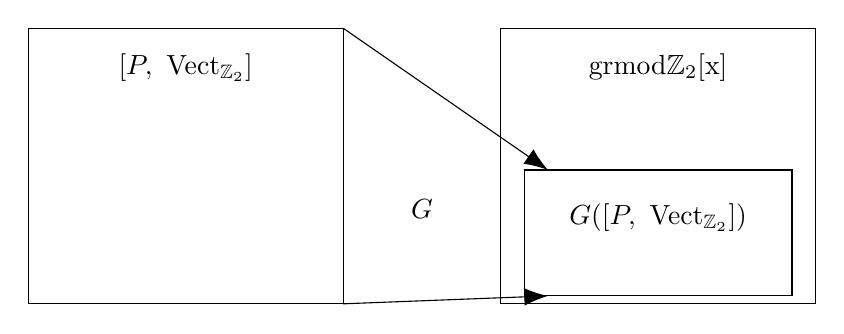
\begin{tikzpicture}
    \node at (0, 1) {$\Fun{P}{\Vect_{\mathbb{Z}_2}}$};
    \node at (6, 1) {$\grmodZ$};
    \node at (3, -0.8) {$G$};
    \node at (6, -0.9) {$G(\Fun{P}{\Vect_{\mathbb{Z}_2}})$};
    \draw (-2,-2) rectangle (2,1.5);
    \draw (4,-2) rectangle (8,1.5);
    \draw (4.3,-1.9) rectangle (7.7,-0.3);
    \draw [-{Latex[length=3mm]}]  (2,-2) -- (4.6, -1.9);
    \draw [-{Latex[length=3mm]}]  (2,1.5) -- (4.6, -0.3);
\end{tikzpicture}\notag
\end{equation}
\section{議論 discussion}
本稿では, パーシステントホモロジーの二つの代数的解釈の関係性の明示を試みた. 結果として充満忠実関手により圏同値を示すことができた. しかし, $\grmodZ$と$\grmodZ$の$G$に関する部分圏の関係性を明示することが課題として残った. また, [4]での次数付き加群としての解釈([4], p.111)と少し異なる部分が存在する. それは$G(V)=\bigoplus V_i$の定義で$i>n$のとき0としたところ, [4]では$V_n$としていることである. ただし双方
の定義は, $i>n$のとき情報が増えないという点で一致しており, この関係は同値関係にあるものと予想している.


\begin{thebibliography}{9}
    \bibitem{1}Dong Quan Ngoc Nguyen, Phuong Dong Tan Le, Lin Xing and Lizhen Lin. "A topological characterization of DNA sequences based on chaos geometry and persistent homology" International Conference on Computational Science and Computational Intelligence (CSCI), p.1599-1605, 2022
    \bibitem{2} Marian Gidea and Yuri Katz. "Topological data analysis of financial time series: Landscapes of crashes" Physica A: Statistical Mechanics and its Applications, Vol. 491, p.820-834, 2018
    \bibitem{3} 池祐一, E.G.エスカラ, 大林一平, 鍛冶静雄 (2023), 『位相的データ解析から構造発見へ -パーシステントホモロジーを中心に』, サイエンス社
    \bibitem{4} 平岡裕章 (2013), 『タンパク質構造とトポロジー -パーシステンホモロジー群入門』, 共立出版
    \bibitem{5} T.レンスター (2014), 『ベーシック圏論 -普遍性からの速習コース』(斎藤恭司監修, 土岡俊介訳), 丸善出版
    
\end{thebibliography}
\section*{謝辞}
本稿を書き上げるため協力いただいた全ての人に感謝を述べたい. 指導教員 Emerson Gaw Escolar 先生, 同研究室の方々, 共に切磋琢磨した同級生に謝意を表する.


\end{document}

